\documentclass[letterpaper]{article}
\usepackage[draft]{aaai2026}
\usepackage{times}
\usepackage{helvet}
\usepackage{courier}
\usepackage{graphicx}
\usepackage{natbib}
\usepackage{caption}
\frenchspacing
\setlength{\pdfpagewidth}{8.5in}
\setlength{\pdfpageheight}{11in}
\usepackage{amsfonts}
\usepackage{pifont}
\usepackage{algorithm}
\usepackage{algorithmic}
\usepackage{amsmath}
\usepackage{xcolor}
\usepackage{booktabs}
\usepackage{multirow}
\usepackage{siunitx}
\usepackage{makecell}
\usepackage{newfloat}
\usepackage{listings}
\DeclareCaptionStyle{ruled}{labelfont=normalfont,labelsep=colon,strut=off}
\lstset{
	basicstyle={\footnotesize\ttfamily},
	numbers=left,numberstyle=\footnotesize,xleftmargin=2em,
	aboveskip=0pt,belowskip=0pt,
	showstringspaces=false,tabsize=2,breaklines=true}
\floatstyle{ruled}
\newfloat{listing}{tb}{lst}{}
\floatname{listing}{Listing}
\pdfinfo{
/TemplateVersion (2026.1)
}
\newcommand{\E}{\mathbb{E}}
\newcommand{\N}{\mathbb{N}}
\newcommand{\R}{\mathbb{R}}
\newcommand{\Q}{\mathbb{Q}}
\newcommand{\Z}{\mathbb{Z}}
\newcommand{\tp}{\mathsf{T}}
\RequirePackage{caption}
\usepackage{epigraph}
\usepackage[utf8]{inputenc}
\usepackage[T1]{fontenc}
\usepackage{url}
\usepackage{booktabs}
\usepackage{amsfonts}
\usepackage{nicefrac}
\usepackage{microtype}
\usepackage{xcolor}
\usepackage{amsthm}
\usepackage{amsmath}
\usepackage{amsfonts}
\usepackage{amssymb}
\usepackage{amsthm}
\usepackage{cuted}
\usepackage{enumitem}
\usepackage{url}
\pagestyle{plain}
\newcommand{\pr}{\mbox{\sf P}}
\newcommand{\ex}{{\bf\sf E}}
\newcommand{\var}{\mbox{\sf Var}}
\newcommand{\sd}{\mbox{\sf sd}}
\newcommand{\cv}{\mbox{\sf cv}}
\newcommand{\pdf}{\mbox{\sf pdf}}
\newcommand{\spectrum}{{\sigma\,}}
\newcommand\Complex{\mathbb C}
\newcommand{\weakto}{\rightharpoonup}
\def\bsk{\bigskip\noindent}
\def\ssk{\medskip\noindent}
\def\hsk{\smallskip\noindent}
\newcommand{\evt}{{\cal E}}
\newcommand{\bS}{{\bf S}}
\newcommand{\bbS}{{\mathbb S}}
\newcommand{\bs}{{\bf s}}
\newcommand{\bB}{{\bf B}}
\newcommand{\bI}{{\bf I}}
\newcommand{\bZ}{{\mathbb Z}}
\newcommand{\bu}{{\bf u}}
\newcommand{\bn}{{\bf n}}
\newcommand{\bb}{{\bf b}}
\newcommand{\bx}{{\bf x}}
\newcommand{\bd}{{\bf d}}
\newcommand{\bk}{{\bf k}}
\newcommand{\bg}{{\bf g}}
\newcommand{\bh}{{\bf h}}
\newcommand{\bp}{{\bf p}}
\newcommand{\be}{{\bf e}}
\newcommand{\by}{{\bf y}}
\newcommand{\bz}{{\bf z}}
\newcommand{\bw}{{\bf w}}
\newcommand{\rk}{{\bf r}}
\newcommand{\bzm}{{\bf Z}_+^m}
\newcommand{\tndi}{\rightarrow\infty}
\newcommand{\call}{{\mathcal L}}
\newcommand{\calm}{{\mathcal M}}
\newcommand{\calb}{{\mathcal B}}
\newcommand{\calB}{{\mathcal B}}
\newcommand{\calc}{{\mathcal C}}
\newcommand{\calp}{{\mathcal P}}
\newcommand{\calP}{{\mathcal P}}
\newcommand{\calq}{{\mathcal Q}}
\newcommand{\calQ}{{\mathcal Q}}
\newcommand{\calg}{{\mathcal G}}
\newcommand{\calk}{{\mathcal K}}
\newcommand{\cals}{{\mathcal S}}
\newcommand{\calh}{{\mathcal H}}
\newcommand{\calS}{{\mathcal S}}
\newcommand{\calI}{{\mathcal I}}
\newcommand{\calJ}{{\mathcal J}}
\newcommand{\calstoi}{{\mathcal S}_{> i}}
\newcommand{\calsjto}{{\mathcal S}_{j>}}
\newcommand{\calsito}{{\mathcal S}_{i >}}
\newcommand{\mtp}{{\mathfrak P}}
\newcommand{\cala}{{\mathcal A}}
\newcommand{\calA}{{\mathcal A}}
\newcommand{\calf}{{\mathcal F}}
\newcommand{\calF}{{\mathcal F}}
\newcommand{\caln}{{\mathcal N}}
\newcommand{\calx}{{\mathcal X}}
\newcommand{\cald}{{\mathcal D}}
\newcommand{\calD}{{\mathcal D}}
\newcommand{\calv}{{\mathcal V}}
\newcommand{\ra}{\rightarrow}
\newcommand{\Ra}{\Rightarrow}
\newcommand{\imp}{\Rightarrow}
\newcommand{\callRa}{\calleftrightarrow}
\newcommand{\subs}{\subseteq}
\newcommand{\stle}{\le_{\rm st}}
\newcommand{\abk}{{\bf (a,b,k)}}
\newcommand{\grad}{{\rm grad\,}}
\newcommand{\hti}{{\tilde h}}
\newcommand{\tL}{{\tilde L}}
\newcommand{\wh}{\widehat}
\newcommand{\rinv}{R^{\mbox{\small -\tiny 1}}}
\newcommand{\pre}{\preceq}
\newcommand{\Bbar}{\overline{B}}
\newcommand{\ub}{\underline{b}}
\newcommand{\starti}{\parindent0pt\it}
\newcommand{\startb}{\parindent0pt\bf}
\newcommand{\mc}{\multicolumn}
\newcommand{\lrge}{\ge_{\rm lr}}
\newcommand{\lrle}{\le_{\rm lr}}
\newcommand{\hati}{{\hat i}}
\newcommand{\diag}{{\rm diag}\,}
\newcommand{\vect}{{\rm vect}\,}
\def\R{\mathbb{R}}
\def\ex{\mathbb{E}}
\def\ep{\epsilon}
\newcommand{\norm}[1]{\left\Vert#1\right\Vert}
\newcommand{\abs}[1]{\left\vert#1\right\vert}
\newcommand{\set}[1]{\left\{#1\right\}}
\newcommand{\Real}{\mathbb R}
\newcommand{\Natural}{\mathbb N}
\newcommand{\eps}{\varepsilon}
\newcommand{\To}{\longrightarrow}
\newcommand{\BX}{\mathbf{B}(X)}
\newcommand{\bbP}{\mathbb P}
\newcommand{\bbQ}{\mathbb Q}
\newcommand{\bbQP}{{\mathbb Q}\times{\mathbb P}}
\newcommand{\lP}{L_\bbP}
\newcommand{\lQ}{L_\bbQ}
\newcommand{\lQP}{L_{\bbQ\times\bbP}}
\newcommand{\Sample}{\Sigma}
\newcommand{\Proj}{\Pi}
\newcommand{\Hamil}{\mathcal H}
\newcommand{\Hamiltonian}{\mathbf H}
\newcommand{\bbg}{\mathbf g}
\newcommand{\bbf}{\mathbf f}
\newcommand{\bbh}{\mathbf h}
\newcommand{\bbw}{\mathbf w}
\newcommand{\bbW}{\mathbf W}
\newcommand{\bbr}{\mathbf r}
\newcommand{\bbU}{\mathbf U}
\newcommand{\bbV}{\mathbf V}
\newcommand{\al}{\alpha}
\newcommand{\bet}{\beta}
\newcommand{\g}{\lambda}
\newcommand{\ga}{\gamma}
\newcommand{\dt}{\delta}
\newcommand{\Dt}{\Delta}
\newcommand{\la}{\lambda}
\newcommand{\lam}{\lambda}
\newcommand{\Lam}{\Lambda}
\newcommand{\sig}{\sigma}
\newcommand{\s}{\sigma}
\newcommand{\om}{\omega}
\newcommand{\Om}{\Omega}
\newcommand{\ta}{\theta}
\newcommand{\Th}{\Theta}
\newcommand{\bmr}{\boldsymbol r}               \newcommand{\bmt}{\boldsymbol t}               \newcommand{\bmu}{\boldsymbol\mu}
\newcommand{\const}{{\rm const\,}}
\newcommand{\tcb}[1]{{\textcolor{blue}{#1}}}
\newcommand{\tcr}[1]{{\textcolor{red}{#1}}}
\newcommand{\tcw}[1]{{\textcolor{brown}{#1}}}
\newtheorem{defn}{Definition}
\newtheorem{pro}{Proposition}
\newtheorem{thm}{Theorem}[section]
\newtheorem{lem}{Lemma}[section]
\newtheorem{rem}{Remark}[section]
\newtheorem{asm}{Assumption}
\newtheorem{cor}{Corollary}
\newtheorem{clm}{Claim}
\newtheorem{exm}{Example}
\newtheorem*{exm*}{Example}
\newcommand{\bbQQ}{{\bbQ\times\bbQ}}
\newcommand{\bbPP}{{\bbP\times\bbP}}
\newcommand{\LP}{L_\bbP}
\newcommand{\LQ}{L_\bbQ}
\newcommand{\LQP}{L_{\bbQ\times\bbP}}
\newcommand{\bbt}{{2}}
\newcommand{\Lt}{{L^\bbt}}
\newcommand{\LPt}{{L_\bbP^\bbt}}
\newcommand{\LQt}{{L_\bbQ^\bbt}}
\newcommand{\LQPt}{{L_{\bbQ\times\bbP}^\bbt}}
\newcommand{\DN}{{\mathbf D}^\N}
\newcommand{\bbp}{\mathfrak{p}}
\newcommand{\bbq}{\mathfrak{q}}
\newcommand{\hs}{{h^*}}
\newcommand{\cTs}{{\cT^\dag}}
\newcommand{\supp}{\rm supp\,}
\newcommand{\suppQ}{\mathfrak{Q}}
\newcommand{\suppP}{\mathfrak{P}}
\newcommand\scpr[2]{\langle #1, #2 \rangle}
\newcommand\scprf[2]{\langle #1, #2 \rangle_{\bbf}}
\newcommand\scprif[2]{\langle #1, #2 \rangle_{1/\bbf}}
\newcommand\sinc{{\rm sinc}}
\newcommand{\cP}{\mathcal{P}}
\newcommand{\cQ}{\mathcal{Q}}
\newcommand{\cT}{\mathcal{T}}
\newcommand{\cS}{\mathcal{S}}
\newcommand{\cL}{\mathcal{L}}
\newcommand{\cK}{\mathcal{K}}
\newcommand{\cD}{\mathcal{D}}
\newcommand{\cA}{\mathcal{A}}
\newcommand{\cB}{\mathcal{B}}
\newcommand{\cH}{\mathcal{H}}
\newcommand{\cC}{\mathcal{C}}
\newcommand{\cN}{\mathcal{N}}
\newcommand{\cM}{\mathcal{M}}
\newcommand{\Mat}{\mathcal{M}}
\newcommand{\tr}{{\rm Tr}}
\newcommand{\Id}{{\rm I}}
\setcounter{secnumdepth}{0}
\title{In-Context Reinforcement Learning via Communicative World Models}
\author{
    Fernando Martinez-Lopez\textsuperscript{\rm 1}\thanks{This research was supported by the AI Summer Research Fellowship from Fordham University's GSAS}, Tao Li\textsuperscript{\rm 2}\thanks{Corresponding author}, Yingdong Lu\textsuperscript{\rm 3}, Juntao Chen\textsuperscript{\rm 1}
}
\affiliations{
    \textsuperscript{\rm 1}Department of Computer and Information Sciences, Fordham University\\
    \textsuperscript{\rm 2} Department of Systems Engineering, City University of Hong Kong\\
    \textsuperscript{\rm 3} IBM Research\\
    \textsuperscript{\rm 1}\{fmartinezlopez, jchen504\}@fordham.edu, \textsuperscript{\rm 2}li.tao@cityu.edu.hk, \textsuperscript{\rm 3}yingdong@us.ibm.com
}
\iffalse
\title{My Publication Title --- Single Author}
\author {
    Author Name
}
\affiliations{
    Affiliation\\
    Affiliation Line 2\\
    name@example.com
}
\fi
\iffalse
\title{My Publication Title --- Multiple Authors}
\author {
    First Author Name\textsuperscript{\rm 1},
    Second Author Name\textsuperscript{\rm 2},
    Third Author Name\textsuperscript{\rm 1}
}
\affiliations {
    \textsuperscript{\rm 1}Affiliation 1\\
    \textsuperscript{\rm 2}Affiliation 2\\
    firstAuthor@affiliation1.com, secondAuthor@affilation2.com, thirdAuthor@affiliation1.com
}
\fi
\begin{document}
\maketitle
\begin{abstract}
Reinforcement learning (RL) agents often struggle to generalize to new tasks and contexts without updating their parameters, mainly because their learned representations and policies are overfit to the specifics of their training environments. To boost agents' in-context RL (ICRL) ability, this work formulates ICRL as a two-agent emergent communication problem and introduces CORAL (Communicative Representation for Adaptive RL), a framework that learns a transferable communicative context by decoupling latent representation learning from control. In CORAL, an Information Agent (IA) is pre-trained as a world model on a diverse distribution of tasks. Its objective is not to maximize task reward, but to build a world model and distill its understanding into concise messages. The emergent communication protocol is shaped by a novel Causal Influence Loss, which measures the effect that the message has on the next action. During deployment, the previously trained IA serves as a fixed contextualizer for a new Control Agent (CA), which learns to solve tasks by interpreting the provided communicative context. Our experiments demonstrate that this approach enables the CA to achieve significant gains in sample efficiency and successfully perform zero-shot adaptation with the help of pre-trained IA in entirely unseen sparse-reward environments, validating the efficacy of learning a transferable communicative representation.\footnote{Code and experimental details are available at \url{https://github.com/fernando-ml/CORAL}.}
\end{abstract}
\section{Introduction}
Pursuing a generalist agent, which is capable of solving a wide range of tasks with minimal intervention, has long been considered one of the central challenges of reinforcement learning (RL) and artificial intelligence (AI) at large \cite{reed22gato}. A general-purpose RL algorithm spares one from hand-crafting domain-specific inductive biases in training \cite{silver19bias,li25piprl} and enables fast adaptation to unseen and complex environments \cite{tao22confluence}.
Most recently, substantial effort has been dedicated to two distinct research thrusts targeting RL generalization: in-context reinforcement learning (ICRL) \cite{laskin2023incontext} and world models (WM) \cite{silver20wm, hafner25worldmodel}. The key idea behind ICRL is to condition the RL policy on some context variables in addition to the state observations. The adaptation power originates from the agent's response to the emerging context extracted from the past interactions \cite{laskin2023incontext, tao23sce}, which reveals task-related information that improves generalization \cite{tao23cola}. The defining characteristic of ICRL is that the in-context policy improvement is purely context-driven and does not rely on policy model updates as in gradient-based meta RL \cite{finn17maml, fallah2021convergence, tao2024meta, pan-tao25meta-lqr}.
However, most recent ICRL approaches condition on past trajectories using the transformer architecture \cite{vaswani2017attention} but typically do not understand the underlying task dynamics. Consequently, their performance depends largely on the quality of offline datasets \cite{chen2021dt}, which limits generalization beyond the distribution of training contexts \cite{chen2024deep_survery}. In contrast, world models (WMs), typically generative models, aim to equip agents with a structured understanding of the environment dynamics and reward feedback, which allows agents to predict how the environment will evolve in response to their actions, even those rarely seen in the pre-training dataset  \cite{hafnerdream, hafner25worldmodel}.
From an ICRL perspective, the latent representation learned by the WM, which captures the dynamics and task reward, provides a context for RL agents when deployed in a variety of environments. Our intuition is that WMs are more suitable as contextualizersthan vanilla, self-supervised trained transformers, leading to a subsequent reinforcement pre-training in ICRL with improved generalizability \cite{moeini2025survey}. In summary, while ICRL facilitates context-driven adaptation, it often lacks understanding of the environment dynamics, making the generalization fragile. While WMs learn such dynamics, the learned representations, however, are often entangled with task-specific policy learning, which can lead to representations that are overly specialized and less transferable, and the objective mismatch between representation and policy learning \cite{eysenbach2022joint}.
\begin{figure*}[th]
\vspace{-5pt}
    \centering
    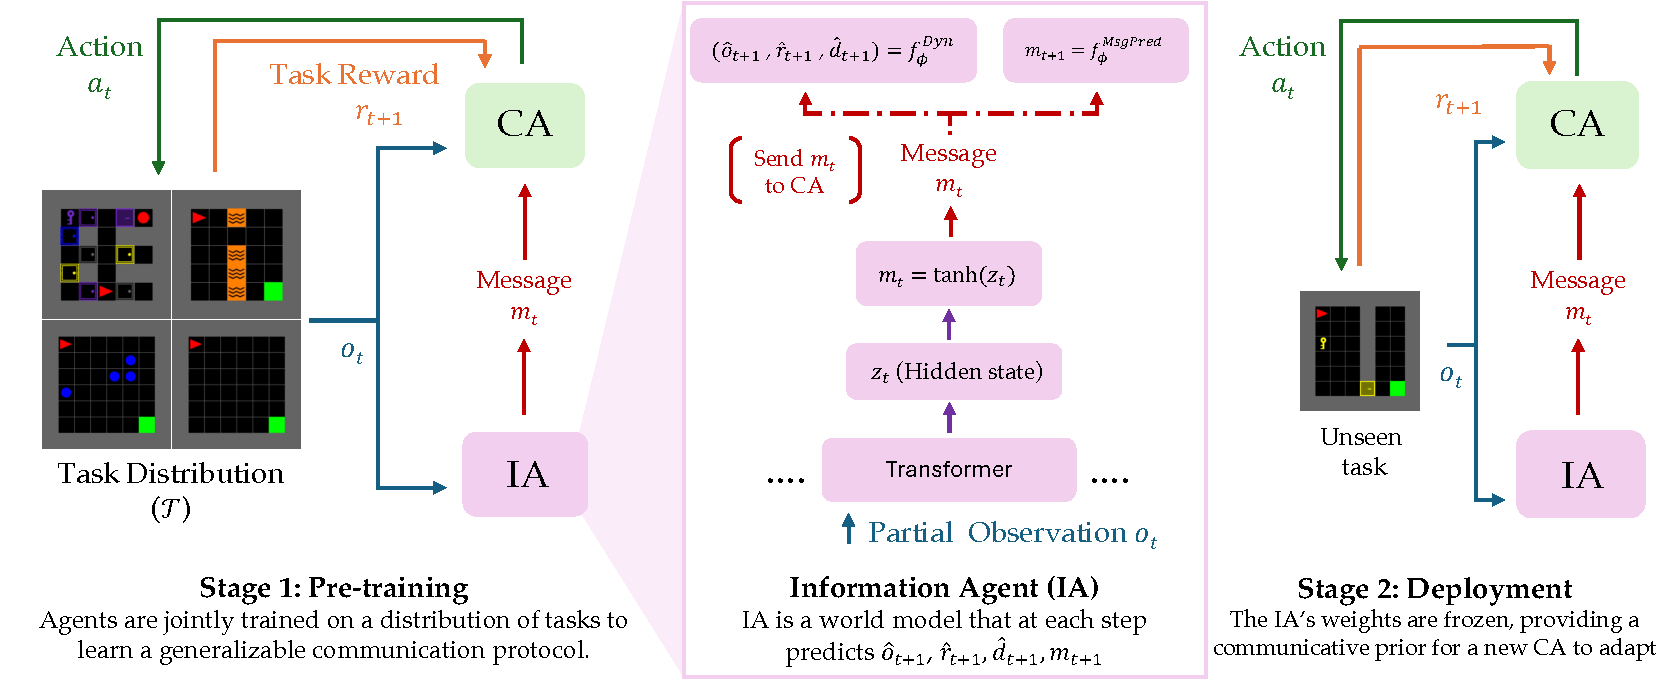
\includegraphics[width=0.9\linewidth]{Figures/CORAL2.pdf}
    \caption{\textbf{Overview of the CORAL framework for learning and deploying a communicative prior.} \textbf{(Left) Pre-training.} An Information Agent (IA, parameterized by $\phi$) and a Control Agent (CA, parameterized by $\theta$) are trained jointly on a distribution of tasks $\mathcal{T}$. The IA, a Transformer-based model detailed in the center panel, processes a partial observation $o_t$ to produce a message $m_t$. The CA is a standard PPO agent that conditions its policy on both $o_t$ and $m_t$ to select an action $a_t$, learning from the task reward $r_{t+1}$. The IA is trained with a set of self-supervised and communication-based objectives. The pre-trained IA is frozen and paired with a new, randomly initialized CA. \textbf{(Right) Deployment}. The IA provides a continuous stream of messages, acting as a communicative prior to accelerate the CA's adaptation to an unseen task.}
    \label{fig:CORAL-design}
    \vspace{-5pt}
\end{figure*}
To address WMs' limitation above and make it better suited for ICRL, we propose to separate the representation learning from the policy learning and introduce the Communicative Representation for Adaptive RL (CORAL) framework, illustrated in Fig.~\ref{fig:CORAL-design}. CORAL decouples the representation and policy learning and formulates ICRL as a two-agent emergent communication problem \cite{lowe2019pitfalls, zhu2024survey}, where a world model, called Information Agent (IA), aims to understand the environment dynamics and task reward, and communicate its understanding through latent representations to a Control Agent (CA), parameterized by a neural network policy model. CORAL's novelty lies in that IA, parameterized by a transformer, generates its messages considering three aspects: 1) dynamics awareness, messages encode the predictions of future consequences, 2) temporal coherence, consecutive messages in the same context must be alike to ensure consistency, and 3) in-context communication effectiveness, the control policy conditioned on messages yields higher return than without.
Our contributions are summarized below, and we postpone the discussion on related works to the end. 1) \textbf{Formulation}: We model a single-agent ICRL problem as a two-agent emergent communication where the world model (information agent) learns how to communicate the learned dynamics to the control agent. 2) \textbf{Hybrid Training}: since the information and control agents face distinct objectives, they are pre-trained differently. The transformer-based IA adopts a self-supervised training with three heads using three losses targeting dynamic awareness, temporal coherence, and communication effectiveness, while the CA adopts proximal policy optimization for reinforcement pre-training. 3) \textbf{Empirical Validation}: We provide extensive empirical validation in partially observable sparse-reward environments, where CORAL yields improved sample-efficiency (5X faster than vanilla WM) and facilitates zero-shot generalization.
\section{Preliminaries}
We formulate RL tasks as Partially Observable Markov Decision Processes (POMDP)~\cite{kaelbling1998planning}. The agent learns a policy $\pi$ to select actions $a_t$ based on a sequence of partial observations $o_t$, as the true environment state $s_t$ is not directly accessible. The agent's objective is to maximize the expected discounted return $\E_{\pi}[\sum_{t=1}^\infty\gamma^{t-1} r_{t}]$, where $r_t$ is the reward received after taking $a_t$ and $\gamma$ is the discount factor. We define the value function, parameterized by a neural network, as  $V_\theta(o_t) =\E_{\pi}[\sum_{k=0}^\infty \gamma^{k}r_{t+k}|o_t ]$.
The emergent communication between two agents in POMDP under cheap-talk setting is mathematically a communication game \cite{crawford82signaling,lowe2019pitfalls, tao23pot, yang-tao25misinformation}. In addition to the control agent whose setup is the same as above, an information agent adopts a communication policy $\pi^{\textsc{ia}}(\cdot|o_t)$, from which a message $m_t$ is drawn. The communication is cheap because $m_t$ does not incur cost to any agent nor influence state transition. In this case, the control agent's policy become $\pi^{\textsc{ca}}(\cdot|o_t, m_t)$, which still aims to maximizes the cumulative rewards, whereas the IA's return, fully determined by CA's actions, may share the same objective as CA's \cite{sukhbaatar16comm} or a totally different one \cite{crawford82signaling, tao23pot}.
\section{Methodology}
The challenge of enabling intelligent agents to generalize and rapidly adapt to new situations is a central pursuit in reinforcement learning. Standard end-to-end paradigms, where a single reward signal shapes a monolithic network, can be remarkably effective~\cite{mnihHumanlevelControlDeep2015} but often yield representations that are overly specialized to the training task, hindering generalization. This has motivated research into decoupled approaches where general-purpose representations are learned via self-supervised objectives~\cite{pmlr-v139-stooke21a, schwarzer2021pretraining}. While these methods can produce robust features, they may not be optimally tailored for the specific downstream control task.
\paragraph{Overview} We propose CORAL (Communicative Representation for Adaptive RL), a framework that navigates a principled middle ground. CORAL conceptualizes the learning problem through a functional separation of representation and control. A dedicated Information Agent (IA) learns a dynamics model, while a separate Control Agent (CA) is tasked with maximizing rewards. This structure allows the IA's learned protocol to serve as a powerful contextual prior for the CA, enabling rapid in-context adaptation.
CORAL's design is centered on the asymmetric learning objectives of the two agents. The CA is a standard RL agent driven by extrinsic task reward, whereas the IA's learning objective is deliberately decoupled from this reward signal. The IA is responsible for building a predictive model of the environment's dynamics and distilling this understanding into a communicative representation. For this decoupling to be effective, the IA's communication must be explicitly shaped to benefit the CA's control policy.
This is achieved through a composite loss that combines self-supervised dynamics modeling with a causal influence objective. The IA is trained to predict future observations, rewards, and termination signals, which grounds its internal representations in the physical reality of the environment. Simultaneously, its Causal Influence Loss shapes the content of its messages. This objective encourages the IA to generate communications that produce a large, decisive shift in the CA's policy, but only when that shift is correlated with high-utility outcomes. The utility is measured by a hybrid signal combining the long-term Generalized Advantage Estimate (GAE) with the immediate change in the CA's own value estimate, effectively teaching the IA to communicate information that is both immediately and prospectively useful. This principled separation allows the IA to form a general representation, which serves as a powerful, pre-trained communicative prior during deployment.
\subsection{CORAL Agents and Emergent Communication}
CORAL is realized through two distinct neural network architectures that interact at each timestep $t$. Both agents receive the same partial observations  $o_t \in \mathbb{R}^{D_{\text{obs}}}$, but serve specialized roles. The Information Agent (IA), parameterized by $\phi$, is designed to integrate historical information and model environmental dynamics. It is implemented as a  Transformer-based architecture~\cite{vaswani2017attention} that operates on a context window of the most recent $L$ observation embeddings, denoted as $c_t = (e_{t-L+1}, \ldots, e_t)$. At each timestep, the observation $o_t$ is transformed into an embedding $e_t$ through a linear layer, updating the context window via a sliding buffer. The sequence $c_t$ is then processed through a series of self-attention and feed-forward layers with residual connections, allowing every token in the context to attend to every other. This produces a sequence of contextualized output vectors.
We extract the final output vector, $z_t$, which corresponds to the most recent observation, as the IA's state representation. This architecture allows the IA to reason about temporal dependencies within its observation history when constructing its communication. The message is then generated by a final linear layer with a $\tanh$ activation: $m_t = \tanh(f_{\phi}^{\text{Msg}}(z_t))$. The $\tanh$ function bounds the message vector, stabilizing the communication channel. Crucially, the IA's learning is not directly driven by extrinsic task rewards but by a set of self-supervised and communication-centric objectives.
The Control Agent (CA), parameterized by $\theta$, is responsible for action and control. It is a standard actor-critic agent trained with Proximal Policy Optimization (PPO)~\cite{schulman2017proximal}. Its policy $\pi_{\theta}(\cdot|o_t, m_t)$ and value function $V_{\theta}(o_t, m_t)$ are conditioned on both its observation and the message. Its sole objective is to maximize the task reward.
\subsection{Pre-training the Communicative Representation}
The parameters $\phi$ and $\theta$ of both agents are optimized jointly in pre-training. The learning objectives are designed to produce an IA that understands the world's dynamics and can communicate that understanding effectively, and a CA that can leverage this communication to solve the task.
\subsubsection{The Information Agent as a Communicative World Model}
The IA is trained via a composite self-supervised loss function, $\mathcal{L}(\phi)$, that does not depend directly on the extrinsic task reward. It combines objectives for world dynamics modeling, message consistency, and communicative efficacy.
\begin{equation*}
    \mathcal{L}(\phi) = \lambda_{\text{Dyn}} \mathcal{L}_{\text{Dyn}}(\phi) + \lambda_{\text{Coh}} \mathcal{L}_{\text{Coh}}(\phi) + \lambda_{\text{Causal}} \mathcal{L}_{\text{Causal}}(\phi).
\end{equation*}
\textbf{Dynamics Awareness Loss ($\mathcal{L}_{\text{Dyn}}$):} This objective grounds the IA's representations by training it to predict the consequences of the CA's actions. Using the message $m_t$ and the action $a_t$ taken by the CA, the IA predicts the next observation $\hat{o}_{t+1}$, reward $\hat{r}_{t+1}$, and termination probability $\hat{d}_{t+1}$; see Appendix~\ref{appendix:hyperparameters_and_setup} for details.
\begin{align*}
    &\mathcal{L}_{\text{Dyn}}=\\
&\mathbb{E}_t [  \underbrace{\| \hat{o}_{t+1} - o_{t+1} \|^2}_{\text{\ding{172}}} + \underbrace{(\hat{r}_{t+1} - r_{t+1})^2}_{\text{\ding{173}}}   +  \underbrace{\text{BCE}(\hat{d}_{t+1}, d_{t+1})}_{\text{\ding{174}}}],
\end{align*}
where predictions are generated by prediction heads ($f_{\phi}^{\text{Dyn}}$) conditioned on the message $m_t$ and action $a_t$: $(\hat{o}'_{t+1}, \hat{r}_{t+1}, \hat{d}_{t+1}) = f_{\phi}^{\text{Dyn}}(m_t, a_t)$. \ding{172} and \ding{173} use mean-square error since observation and action predictions are continuous, whereas \ding{174} considers binary cross-entropy (BCE) loss for probabilistic outputs.
\textbf{Temporal Coherence Loss ($\mathcal{L}_{\text{Coh}}$):} To promote temporal coherence in communication, the IA is also trained to predict the next message $m_{t+1}$ based on the current message $m_t$ through a specific prediction head ($f_{\phi}^{\text{MsgPred}}$) with the loss given by $\mathcal{L}_{\text{Coh}} = \mathbb{E}_t \left[ \| \hat{m}_{t+1} - m_{t+1} \|^2 \right]$, where $\hat{m}_{t+1} = f_{\phi}^{\text{MsgPred}}(m_t, a_t)$. We encourage the message to be a compact representation of the state from which future states (and thus future messages) can be inferred.
\textbf{Causal Influence Loss ($\mathcal{L}_{\text{Causal}}$):} To shape the communication to be effective from the CA's perspective, we introduce an information-theoretic objective inspired by the work on measuring causal influence in emergent communication~\cite{lowe2019pitfalls}. This loss encourages the IA to produce messages that cause a beneficial and decisive shift in the CA's policy. We quantify this per-step shift using a metric we term the Instantaneous Causal Effect (ICE), defined as the Reverse KL Divergence between the CA's policy with and without the message:
\begin{align}
    \text{ICE}_t =D_{\text{KL}}\Big(\pi_{\theta}(\cdot|o_t, \mathbf{0}) \parallel \pi_{\theta}(\cdot|o_t, m_t)\Big). \tag{ICE}
    \label{eq:ice}
\end{align}
Here, $\pi_{\theta}(\cdot|o_t, \mathbf{0})$ is is conditioned on a zero-vector message, representing a non-informative communicative input.
To encourage helpful messages from IA that yield high-return actions, we multiply the ICE by a hybrid utility signal $\mathcal{U}_t$. The signal combines two sources of utility: The first is the GAE~\cite{schulman2015high}, $A_t$, which provides a low-variance estimate of the long-term, empirical advantage of taking an action. It is calculated as the exponentially-weighted average of temporal difference errors: $A_t = \sum_{k=0}^{\infty} (\gamma\lambda)^k \delta_{t+k}$, where $\delta_t = r_{t+1} + \gamma V_{t+1} - V_t$. The second source is the immediate change in the CA's own value estimate, $\Delta V_t = V_{\theta}(o_t, m_t) - V_{\theta}(o_t, \mathbf{0})$. To ensure that both signals contribute on a comparable scale regardless of reward magnitude or the stage of training, we apply z-score normalization, a standard technique for stabilizing policy gradient updates~\cite{schulman2017proximal, ioffe2015batch}. These normalized signals are then combined and clipped to form the final positive utility signal $\mathcal{U}_t$:
$$\mathcal{U}_t = \max\{0, \alpha \cdot \text{norm}(\Delta V_t) + (1-\alpha) \cdot \text{norm}(A_t)\}.$$
The final loss term maximizes the utility-weighted KL divergence over trajectories $\tau$ from the joint policy,
\begin{align*}
    &\mathcal{L}_{\text{Causal}}(\phi) = - \mathbb{E}_{\tau \sim \pi_{\theta, \phi}} \left[\mbox{ } \mathcal{U}_t \cdot \text{ICE}_t\mbox{ } \right].
\end{align*}
The utility signal $\mathcal{U}_t$ is treated as a constant during the optimization of $\phi$ by detaching it from the computation graph. This ensures that the gradient only flows through the KL divergence term, correctly isolating the objective to rewarding the IA for how its message $m_t$ influences the CA's policy, rather than for influencing the value estimates that comprise the utility signal itself.
\subsection{Multi-Environment Training for Generalization}
CORAL aims to produce a communicative prior that is not overfitted to a single task but is instead broadly applicable. It is well-established that deep RL agents can achieve high performance by overfitting to the specific stochasticity of their training environments, yet fail to generalize to slightly different, unseen situations \cite{cobbe2020leveraging}.
To directly address this challenge, our pre-training regime moves beyond single-task optimization and instead trains the CORAL agents on a diverse, discrete set of tasks, $\mathcal{T} = \{\text{env}_1, \ldots, \text{env}_K\}$, that share common entities and dynamics but require different solutions. Our implementation is based on modern, vectorized training within a single process. Inspired by the architectural principles of large-scale distributed agents \cite{espeholt2018impala} and using an implementation pattern similar to high-performance JAX-native frameworks like PureJaxRL \cite{lu2022discovered}, we leverage the `vmap' transformation in JAX \cite{jax2018github} to run N parallel environments simultaneously on a single accelerator.
At the beginning of each rollout, each of the $N$ parallel environment instances is randomly assigned a task from our distribution $\mathcal{T}$. This ensures that every gradient update batch contains a rich mixture of experiences from across the task family. By training on this diverse data stream, we prevent catastrophic forgetting and force the Information Agent to learn an abstract dynamics model, capturing the fundamental rules and entities common across environments rather than memorizing the specifics of any single instance. This multi-task regime is critical for learning a communicative representation that can serve as a truly generalizable prior.
\subsection{Deployment for Rapid In-Context Adaptation}
During deployment, the parameters $\phi$ of the Information Agent are frozen. The IA now functions as a fixed, deterministic module that provides a continuous stream of contextual information. This setup allows us to rigorously test our central hypothesis that the learned communication protocol enables rapid, sample-efficient adaptation for a Control Agent.
We formalize this evaluation through the lens of in-context reinforcement learning \cite{lee2023supervised, laskin2023incontext}. The Control Agent's learning process can be viewed as an inference problem, where it must deduce the optimal policy for a new environment by conditioning on the history of observations and messages that form its context.
\section{Experimental Results}
\begin{figure*}[t]
    \centering
    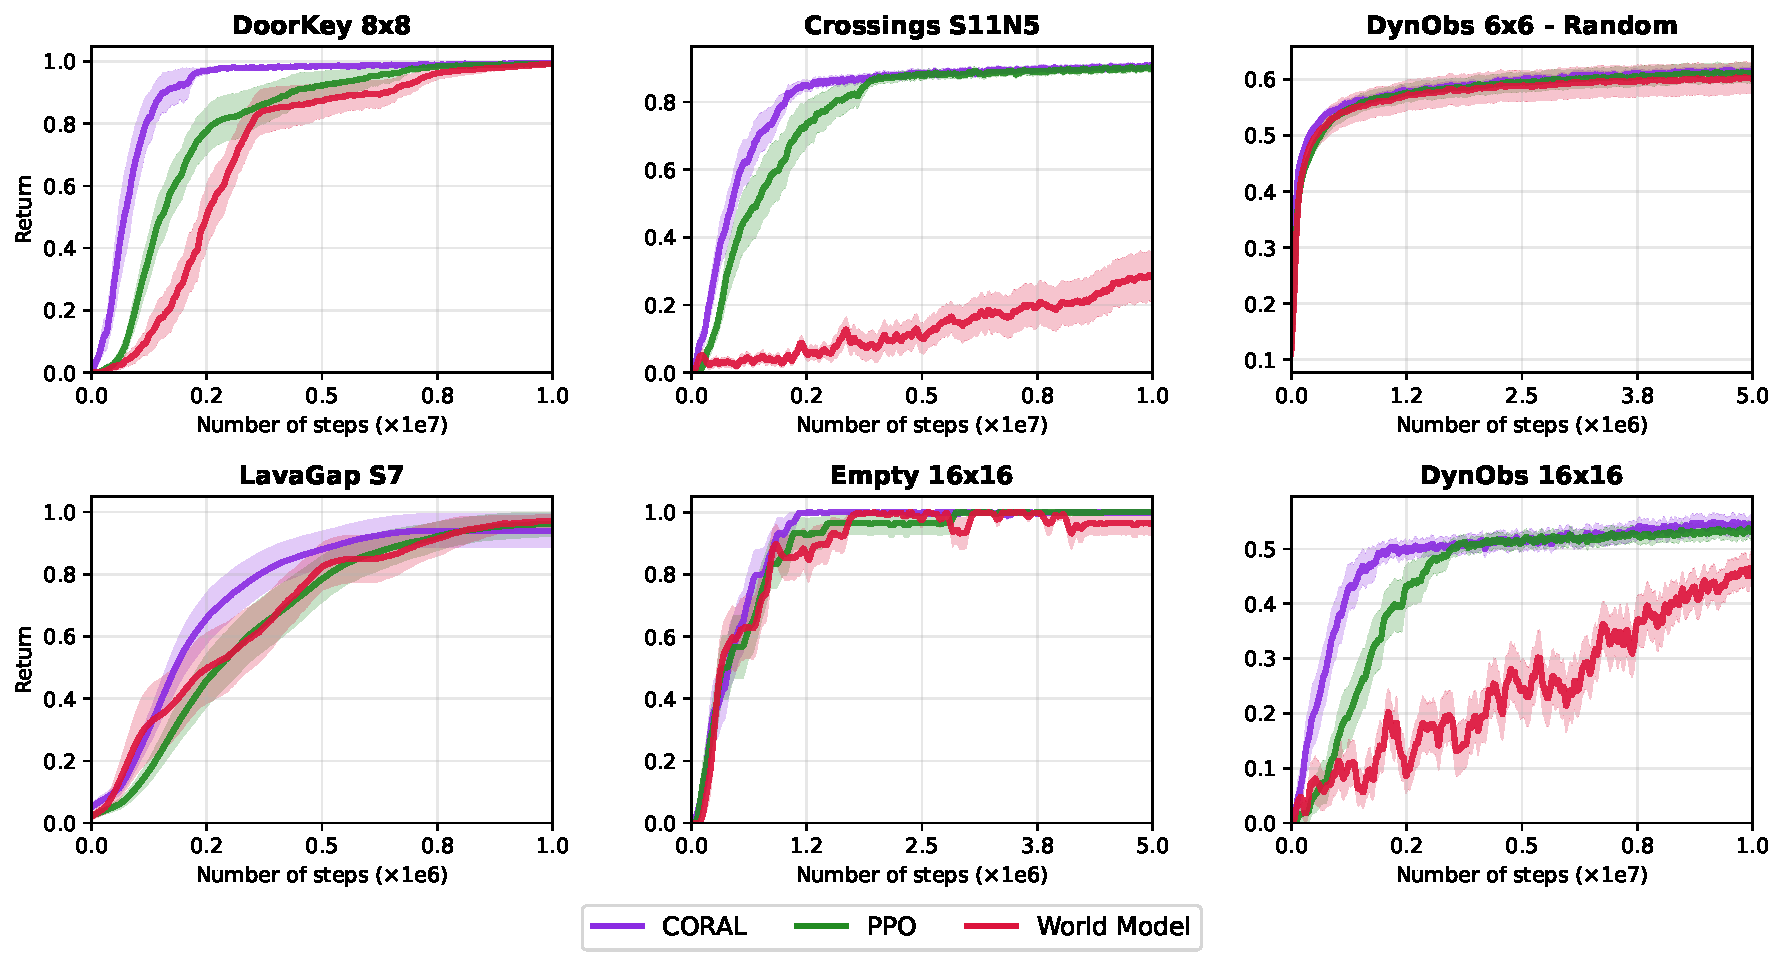
\includegraphics[width=.85\linewidth]{Figures/lc.pdf}
    \vspace{-5pt}
    \caption{\textbf{In-context adaptation with a pre-trained Information Agent.} Learning curves show the mean episodic return ($\pm95\%$ confidence interval) across 30 multiple seeds for a randomly initialized Control Agent paired with a pre-trained, frozen CORAL IA. \textcolor[HTML]{923BE5}{CORAL} demonstrates higher sample efficiency and asymptotic performance compared to a \textcolor[HTML]{339332}{standard PPO} and an \textcolor[HTML]{DD264A}{equivalent World Model} across a variety of unseen environments.}
    \label{fig:learning-curves}
    \vspace{-5pt}
\end{figure*}
We conduct a series of experiments designed to validate our central hypothesis: a pre-trained communicative prior, learned via CORAL, can enable rapid in-context adaptation by providing a rich, task-relevant learning signal in environments where such information is otherwise unavailable. Specifically, we demonstrate that CORAL excels in settings characterized by sparse rewards, partial observability, and long-range dependencies (challenges that are known to impede standard model-free agents). Accordingly, our evaluation is structured to first demonstrate our framework's sample efficiency compared to baselines, then to rigorously test the generalization of its learned protocol to unseen tasks, and finally to analyze the communication itself to verify it is causally responsible for the observed gains.
To this end, we perform experiments on a suite of partially observable grid-world environments using Navix \cite{pignatelli2024navix}, a high-performance JAX-native implementation of MiniGrid \cite{chevalier2023minigrid}. These environments are well-suited for our work as they feature sparse reward and long decision-making horizons challenges. Our pre-training distribution $\mathcal{T}$ is curated to be diverse, including tasks such as Empty, Crossings, DoorKey, LavaGap, DynamicObstacles, and randomized variants (details in Appendix \ref{appendix:hyperparameters_and_setup}). We evaluate generalization ability by deploying agents in larger or more complex unseen versions of these tasks.
To ensure a fair and comprehensive comparison, we evaluate the performance of our CORAL agent against two strong baselines. The first is a standard PPO agent with a feed-forward policy, representing a tabula rasa learning agent, with the same architecture of CORAL's control agent utilized for these experiments. The second is a more powerful baseline we term \textit{World Model} (WM), is a Transformer-based agent whose architecture is identical to our IA. The WM is trained with a composite objective that combines the standard PPO loss for policy and value functions with the same self-supervised self-supervised dynamics-prediction objectives ($\mathcal{L}_{\text{Dyn}}$) used by our IA.
\subsection{Accelerated Control Learning via In-Context Communication}
Our first set of experiments assesses the ability of the pre-trained CORAL Information Agent to accelerate the learning of a new Control Agent from scratch in unseen tasks. In this setting, the IA's parameters are frozen, and it is paired with a randomly initialized CA in a series of unseen evaluation environments. The results presented in Fig.~\ref{fig:learning-curves}, show that the CORAL-guided agent consistently and substantially outperforms both the PPO and world model baseline.
\begin{table*}[bt]
\vspace{-5pt}
\centering
  \begin{tabular}{l c cc cc cc}
    \toprule
    \multirow{2}{*}{Environment} &
    \multirow{2}{*}{Max. Perf} &
    \multicolumn{2}{c}{\textcolor[HTML]{923BE5}{CORAL}} &
    \multicolumn{2}{c}{\textcolor[HTML]{339332}{PPO}} &
    \multicolumn{2}{c}{\textcolor[HTML]{DD264A}{World Model}} \\
      & & TTT & SR & TTT & SR & TTT & SR \\
    \midrule
DoorKey 8x8 & 1.00 & \textbf{1.0 $\pm$ 0.2$^{\dag}$} & 100\% & 2.3 $\pm$ 0.3 & 100\% & 3.0 $\pm$ 0.4 & 89\% \\
Crossings S11N5 & 1.00 & \textbf{1.3 $\pm$ 0.1$^{\dag}$} & 100\% & 1.9 $\pm$ 0.3 & 100\% & 6.9 $\pm$ 1.2 & 19\% \\
DynObs 6x6 - Random & 0.74 & 1.5 $\pm$ 0.2 & 100\% & 1.5 $\pm$ 0.1 & 97\% & \textbf{1.3 $\pm$ 0.1} & 97\% \\
LavaGap S7 & 1.00 & \textbf{0.3 $\pm$ 0.0$^{\dag}$} & 95\% & 0.4 $\pm$ 0.0 & 95\% & 0.4 $\pm$ 0.0 & 94\% \\
Empty 16x16 & 1.00 & \textbf{0.5 $\pm$ 0.1} & 100\% & 0.7 $\pm$ 0.1 & 100\% & \textbf{0.5 $\pm$ 0.1} & 100\% \\
DynObs 16x16 & 0.85 & \textbf{7.0 $\pm$ 0.6$^{\dag}$} & 45\% & 7.9 $\pm$ 0.5 & 36\% & 8.5 $\pm$ 0.7 & 30\% \\
    \bottomrule
  \end{tabular}
\vspace{-5pt}
\caption{Time-to-threshold analysis showing mean timesteps (in millions) ± 95\% confidence interval to reach 90\% maximum performance. SR (\%) is the success rate of runs reaching the threshold. \textbf{Bold} indicate the best method per environment. ${\dag}$ indicates statistically significant improvement over the next-best method (Welch’s t-test, p < 0.05).}
\label{table: TTT}
\vspace{-5pt}
\end{table*}
The learning curves illustrate a significant gain in sample efficiency. In tasks such as \textit{DoorKey 8x8} and \textit{Crossings S11N5}, the CORAL agent reaches near optimal performance in approximately half the time required by the PPO agent. This advantage is particularly pronounced when applied to more complex or larger versions of the training tasks. For instance, in Dynamic Obstacles 16x16 (\textit{DynObs 16x16}), which is a substantially larger and more challenging variant of an environment seen during pretraining, the baselines struggle to make meaningful progress while CORAL makes the CA quickly discover a good policy. This shows that the communicative prior provides effective guidance that is not brittle, allowing a new agent to overcome the exploration challenges inherent in these sparse-reward tasks even as the scale and difficulty of the problem increase.
To quantify this sample efficiency, we perform a time-to-threshold (TTT) analysis, measuring the mean number of timesteps required for each method to reach 90\% of the maximum performance achieved in each environment. As shown in Table~\ref{table: TTT}, CORAL achieves the target performance threshold significantly faster than the baselines in most tasks. For example, in \textit{Doorkey 8x8}, CORAL reaches the target performance in significantly fewer timesteps, achieving the threshold 2.3 times faster than PPO and 3 times faster than the World Model baseline. Similarly, CORAL demonstrates a 1.5-fold speedup over PPO and more than a 5-fold improvement over the World Model baseline in \textit{Crossings S11N5}. The success rate (SR) further highlights CORAL's reliability to solve these tasks; for instance, in the most challenging environment, \textit{DynObs16x16}, CORAL achieves a 25\% relative improvement in SR over PPO and a 50\% over the WM.
The consistent and significant results indicate that the benefit of our framework stem not from the use of a different architecture, but from the communication itself. The performance gap over the PPO baseline demonstrates that the message stream provides a powerful learning signal for exploration in sparse-reward settings. Furthermore, CORAL's superiority over the architecturally-equivalent World Model baseline highlights the benefit of our pre-training strategy. By training the Information Agent with objectives that are not directly tied to maximizing task reward, CORAL develops a more general communication protocol that serves as a more effective in-context learning signal than the task-specific representations learned by the end-to-end model.
\subsection{Integrated In-Context Communication and Control for Zero-Shot Generalization}
Beyond accelerating learning from scratch, we investigate the robustness of the learned policies in a challenging zero-shot transfer setting where no further learning is allowed. For this evaluation, we use the same generalist Information Agent pre-trained on our full task distribution $\mathcal{T}$. We then pre-train the CORAL CA and both baselines on specific, simpler source task (e.g., \textit{DoorKey6x6}). Finally, we freeze all agent parameters and evaluate their performance directly on more complex, unseen target environments (e.g., \textit{DoorKey8x8}). This set of experiments measure how well the learned policy generalize to configurations of increased scale and complexity.
The results, summarized in Table~\ref{table: MaxPerGeneralization}, demonstrate that the CORAL system exhibits superior zero-shot generalization capabilities compared to the baselines. In environments like \textit{DoorKey8x8} and \textit{LavaGapS7}, the pre-trained CORAL agent achieves significantly higher average returns than both the PPO and World Model agents, which were pre-trained on the same source tasks.
\begin{table}[!ht]
\centering
\footnotesize
\setlength{\tabcolsep}{3.1pt}
\begin{tabular}{@{}lccc@{}}
\toprule
\textbf{Environment} & \textcolor[HTML]{923BE5}{CORAL} & \textcolor[HTML]{339332}{PPO} & \textcolor[HTML]{DD264A}{WM} \\
\midrule
DoorKey8x8 &  $\mathbf{0.95\pm9e^{-4}}^{\dag}$ & $0.78\pm6e^{-4}$ & $0.86\pm7e^{-3}$\\
CrossingsS11N5 & $0.45\pm9e^{-3}$ & $\mathbf{0.48\pm8e^{-3}}^{\dag}$ & $0.20\pm5e^{-3}$ \\
DynObs6x6-Rand & $\mathbf{0.64\pm2e^{-3}}^{\dag}$ & $0.43\pm2e^{-3}$ & $0.33\pm7e^{-3}$ \\
LavaGapS7 & $\mathbf{0.77\pm6e^{-3}}^{\dag}$ & $0.63 \pm 6e^{-3}$ & $0.65\pm5e^{-3}$\\
Empty16x16 & $\mathbf{0.90\pm 4e^{-3}}^{\dag}$ & $0.86\pm 3e^{-3}$ & $0.88\pm4e^{-3}$ \\
DynObs16x16 & $\mathbf{0.52\pm6e^{-3}}^{\dag}$ & $0.50\pm5e^{-3}$ & $0.16\pm6e^{-3}$ \\
\bottomrule
\end{tabular}
\vspace{-5pt}
\caption{Zero-shot performance. All agents were pre-trained on simpler source tasks and evaluated with frozen weights. Values are mean episodic return $\pm$ 95\% CI over 1M steps. \textbf{Bold} indicate the best method per environment. ${\dag}$ indicates statistically significant improvement over the next-best method (Welch’s t-test, p < 0.05).}
\label{table: MaxPerGeneralization}
\vspace{-5pt}
\end{table}
\subsection{Analysis of the Emergent Communicative Protocol}
To verify that communication is causally responsible for the observed performance gains, we analyze the protocol's Instantaneous Causal Effect (Eq.~\ref{eq:ice}). A high ICE value indicates that the message is causing a decisive shift in the CA's behavior.
Fig.~\ref{fig:ice} presents the mean and 95\% confidence interval of ICE for CORAL alongside a Control Agent receiving random messages. While the random messages induce a high ICE by acting as a noisy distractor, they result in no meaningful learning. In contrast, CORAL's ICE rises in lockstep with performance as the CA learns to rely on the IA's guidance, and then recedes as the policy is mastered and the message becomes confirmatory. This dynamic, where influence is high during learning and low at convergence, suggests that the CORAL protocol acts as an effective learning catalyst, providing strong guidance only when the agent is uncertain.
\begin{figure*}[bt]
    \centering
    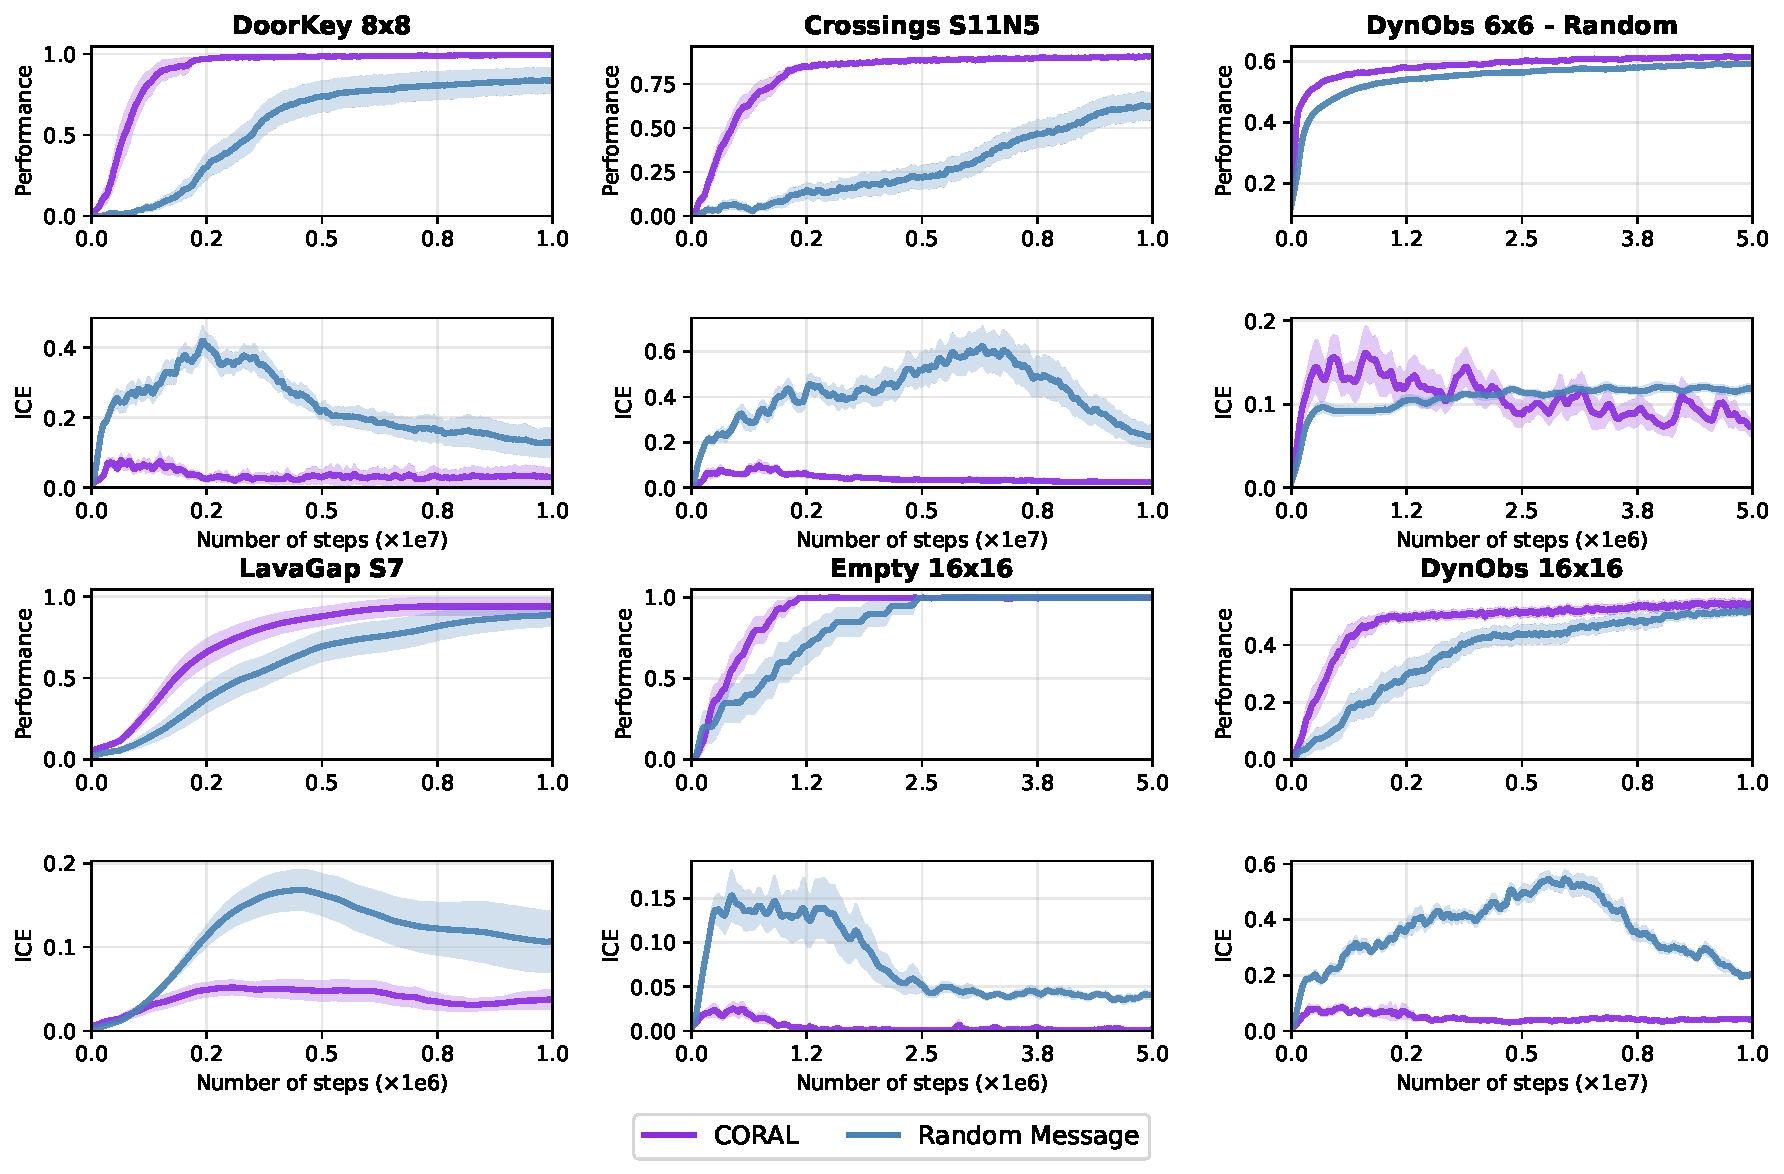
\includegraphics[width=.8\linewidth]{Figures/cic.pdf}
    \caption{\textbf{Analysis of Influence of Communication during In-Context Adaptation.} Learning curves (top row) are paired with the corresponding Instantaneous Causal Effect metric (bottom row) for six unseen environments. ICE measures the per-step policy shift induced by communication (Eq.~\ref{eq:ice}). The \textcolor[HTML]{4682B4}{Random Message} baseline induces a high but unproductive ICE by distracting the agent. Conversely, the  ICE of the \textcolor[HTML]{923BE5}{CORAL} agent rises as the agent learns and then recedes as the policy converges.}
    \label{fig:ice}
    \vspace{-5pt}
\end{figure*}
\section{Related Works}
\label{sec:related}
\paragraph{In-Context Reinforcement Learning} In-context learning, a concept recently popularized by large language models (LLMs) research and applications \cite{dong-etal-2024-survey, tao-qz24symbiotic}, refers to the ability to learn from a few examples in the context and adapt without changing model weights. The idea of few-shot adaptation in ICRL coincides with some earlier works on gradient-free meta learning, where recurrent neural networks, aiming to extract task-specific hidden context from historical interactions, are incorporated into RL training \cite{botvinick16learnRL, abbeel16rl2}.
Thanks to the transformer architecture's sequence modeling capability \cite{vaswani2017attention}, most recent advancements on ICRL leverage transformer and LLMs to extract context variables (e.g., hidden states) from historical trajectories \cite{lee2023supervised, tao23sce, krishnamurthy2024can}. Pre-training in ICRL is the key to its successful in-context adaptation in deployment. Most existing works fall within the categories of (self-) supervised pre-training and reinforcement pre-training \cite{moeini2025survey}.
Supervised pre-training, bearing a similar spirit to imitation learning, encourages agents to find trajectories similar to the current testing task from the offline data and imitate offline actions for better generalization \cite{raparthy24icrl, xu22prompt-dt}. Self-supervised approach, such as decision transformers \cite{chen2021dt, huang2024decision}, utilizes the transformer's auto-regressive generation and predicts the next action based on the predictions on the state observation and reward feedback. Even though some advanced techniques, such as hindsight information matching \cite{furuta21generalDT, tao23sce}, help improve out-of-distribution generalization, the (self-) supervised approaches largely depend on the quality of offline pertaining data.
Our proposed CORAL belongs to the class of reinforcement pre-training, where the policy is not purely extracted from static, offline data but also from live interactions with a variety of environments. Compared with existing works on transformer-based ICRL \cite{bauer23,grigsby2024amago,  wang2024transformers}, which integrates the learning of context into policy learning, our work further decouples the two learning processes and adopts a \textit{hybrid} of supervised pre-training for world model training and reinforcement pre-training for control policies.
\paragraph{World Models}
World models (WMs), typically represented by generative neural networks, serve as the agents' mental models of the world based on what they are able to perceive, which helps agents to conceive future consequences of their actions, thus planning in sequential decision-making \cite{schmidhuber18wm}. Some early efforts focus on building visual WMs using autoencoders and recurrent neural networks (RNNs) \cite{schmidhuber18wm,hafner19a, hafnerdream, hafner25worldmodel}, where WMs predict the next latent representation for planning purposes based on those of previous image inputs. In more structured tasks (e.g., Go),  simple predictive models plus Monte Carlo tree search (MCTS) also yield superior performance \cite{silver20wm, silver21on-off-wm, tao24col, kim-tao25col}.
Our CORAL aligns with the recent trend of transformer-based WMs \cite{micheli2023transformers, robine2023transformerbased} for its improved sample efficiency, compared with RNN-based ones. However, these transformer WMs, like most WMs, directly incorporate the general-purpose dynamics modeling learning with task-specific RL, where agents treat the transformer-generated latent representations as the new state variables.  In contrast, our approach decouples the two learning tasks, and the transformer is only tasked with understanding the shared environment dynamics and communicating them to the control agent as side information or context. Most relevant to ours is \cite{toledocodreamer}, which studies communication-based decentralized WMs. This work proposes to equip each agent with a WM in a multi-agent RL task, where WMs first communicate with each other on future predictions. CORAL, instead, focuses on tackling a single-agent RL from an emergent communication perspective, where the transformer WM is still the mental model without actually optimizing the policy.
\section{Conclusion}
This work introduces CORAL, a framework for learning a communicative prior for in-context reinforcement learning. By pre-training an Information Agent as a communicative world model with objectives decoupled from direct task rewards, we produce a generalizable protocol that effectively guides a new agent's learning process. Our experiments demonstrate that using this pre-trained communicative prior leads to significant gains in sample efficiency and zero-shot performance for new newly initialized agents and in unseen, sparse-reward tasks. This work validates the promise of using emergent communication not merely for coordination, but as a powerful mechanism for rapid adaptation in multi-agent systems.
\bibliography{aaai2026}
\clearpage
\clearpage
\begin{appendix}
\setcounter{secnumdepth}{2}
\section*{Appendix}
\section{Code availability}
\label{appendix:code_availability}
The complete source code for CORAL and the experiments presented in this paper is available at \url{https://github.com/fernando-ml/CORAL} to ensure reproducibility. Our implementation is built in JAX \cite{jax2018github} and leverages significant components, particularly for environment vectorization and training loops, from the PureJaxRL framework \cite{lu2022discovered}\footnote{\url{https://github.com/luchris429/purejaxrl/tree/main}} and Navix \cite{pignatelli2024navix}\footnote{\url{https://github.com/epignatelli/navix}}. While core architectural choices (Appendix~\ref{appendix:hyperparameters_and_setup}) and most hyperparameters for baseline algorithms are consistent with PureJaxRL defaults for Navix.
\section{Limitations and Future Work}
While our work demonstrates the significant potential of using pre-trained communicative priors for in-context adaptation, it also highlights several avenues for future extension.
A primary direction involves the \textbf{scalability and nature of the communication protocol itself}. The fixed-dimensional dense vector used in CORAL, while effective in the studied domains, may not be the most efficient representation for tasks with higher-dimensional inputs or those requiring more compositional reasoning. Future work could explore more structured protocols, such as discrete tokens from a learned vocabulary, to enhance expressivity. Furthermore, our framework operates in the ``cheap talk'' setting where communication is costless~\cite{crawford82signaling,lowe2019pitfalls, tao23pot, yang-tao25misinformation}. Introducing a cost for sending messages could be a valuable extension, potentially encouraging the IA to develop an even more efficient and sparse protocol where it communicates only when the expected utility outweighs the cost.
Another important avenue lies in \textbf{extending the validation of CORAL to more sophisticated domains.} Our experiments show successful transfer and adaptation within the \textit{Navix} family of grid-worlds. An interesting next step is to evaluate the framework's ability to bridge a larger "transfer gap" by pre-training on one class of environments and deploying in fundamentally different ones, such as high-dimensional Atari games or continuous control tasks in MuJoCo. Success in such disparate domains would be a significant step towards truly generalist communicative agents.
Lastly, our framework can be extended to more \textbf{complex multi-agent topologies.} The current work deliberately focuses on an asymmetric agent pair to isolate and study the communicative prior. A natural extension is to scale this to scenarios where a single Information Agent must learn to coordinate multiple, potentially specialized, Control Agents. Future work could also explore settings with bi-directional communication, where all agents are homogeneous and can adopt both speaker and listener roles, moving towards to more applicable real-world coordination problems.
\section{Experiment Setup and Hyperparameters}
\label{appendix:hyperparameters_and_setup}
\paragraph{Software} We used the following software versions:
\begin{itemize}
    \item Python 3.10.18 - Python Software License \url{https://docs.python.org/3/license.html}
    \item CUDA 12.4 - NVIDIA Software License Agreement \url{https://docs.nvidia.com/cuda/eula/index.html}
    \item Jax 0.5.3 - Apache License 2.0 \url{https://github.com/jax-ml/jax}
    \item Flashbax 0.1.2 - Apache License 2.0 \url{https://github.com/instadeepai/flashbax}
    \item Chex 0.1.89 - Apache License 2.0 \url{https://github.com/google-deepmind/chex}
    \item Optax 0.2.4 - Apache License 2.0 \url{https://github.com/google-deepmind/optax}
    \item Flax 0.10.4 - Apache License 2.0 \url{https://github.com/google/flax}
    \item Navix 0.7.0 - Apache License 2.0 \url{https://github.com/epignatelli/navix}
    \item WANDB 0.19.8 - MIT License \url{https://github.com/wandb/wandb}
    \item Gymnax 0.0.8 - Apache License 2.0 \url{https://github.com/RobertTLange/gymnax}
    \item PureJaxRL - Apache License 2.0 \url{https://github.com/luchris429/purejaxrl}
\end{itemize}
\paragraph{Hardware} All experiments were conducted on NVIDIA Tesla V100-PCIE-32GB GPUs. A typical experimental run, consisting of training one algorithm over 30 random seeds for $10^7$ total environment time steps on a Navix environment, completed in approximately 12 to 26 minutes.
\subsection{Pre-training Environment Distribution}
To foster the development of a generalizable transferable communication protocol, our pre-training stage utilizes a diverse distribution of tasks, $\mathcal{T}$. The environments were selected to expose the Information Agent (IA) to a wide range of mechanics, entities, and objectives. This multi-world regime is designed to drive the IA to learn a model of grid-world dynamics, rather than overfitting to the specifics of a single task. The pre-training distribution consists of the following environments:
\begin{itemize}
    \item \textbf{Empty-Random-8x8}: The simplest task, it requires the agent to navigate to a goal in an empty room with randomized start and goal positions. It serves to teach the IA concepts of navigation and goal-directedness in the absence of other factors.
    \item \textbf{GoToDoor8x8}: This task requires the agent to navigate to a specific object (the door) rather than a generic goal tile. This teaches the IA the concept of object-centric goals so it can communicate information about specific entities in the environment.
    \item \textbf{FourRooms}: In this environment, the agent needs to navigate through multiple interconnected rooms. This tests the IA's ability to model and communicate information relevant to planning and navigation with multi-room layouts.
    \item \textbf{CrossingS9N3}: In this environment, the agent must cross a room with static obstacles, teaching the IA to learning about path planning and the semantics of impassable objects like walls.
    \item \textbf{LavaGapS6}: It introduces a "dangerous" terrain type (lava) that the agent must avoid, introducing IA to the concept of environmental constraints and affordances.
    \item \textbf{Dynamic-Obstacles-5x5}: This environment features mobile obstacles (balls) that move randomly. Since this environment is non-stationary, the IA must develop a compelling understanding of the world and communicate about changing states.
    \item \textbf{DoorKey-Random-6x6}: This task introduces the concept of conditional objectives. Here, the agent must first find a key, pick it up, and then use it to open a locked door to reach the goal. For this environment, the IA needs to model a longer sequence of sub-tasks and dependencies between them, and communicate accordingly.
\end{itemize}
\subsection{Neural Network Architectures and Hyperparameters}
CORAL's training and deployment setup and neural network designs are presented in Table \ref{tab:coral_hyperparams}, \ref{tab:coral_ia_architecture}, and \ref{tab:coral_ca_architecture}, respectively.
\begin{table}[!hb]
\centering
\caption{Train \& Deployment Hyperparameters for CORAL. Shared hyperparameters between IA and CA come from Navix's PureJaxRL example for PPO.}
\label{tab:coral_hyperparams}
\resizebox{\linewidth}{!}{
\begin{tabular}{@{}lc@{}}
\toprule
\textbf{Parameter} & \textbf{Value} \\
\midrule
\multicolumn{2}{@{}l}{\textit{ Configuration}} \\
\makecell[l]{Number of parallel environments \\ (Pre-train)} & 128 \\
\makecell[l]{Number of parallel environments \\ (Deploy)} & 16 \\
\makecell[l]{Total timesteps \\ (Pre-train)} & $5 \times 10^7$ \\
\makecell[l]{Total timesteps \\ (Deploy)} & $1 \times 10^7$ \\
Number of steps per rollout & 128 \\
Number of minibatches & 8 \\
Update epochs & 4 \\
\midrule
\multicolumn{2}{@{}l}{\textit{Learning Parameters}} \\
Optimizer & Adam \\
Learning rate (LR) & $2.5 \times 10^{-4}$ \\
Linear learning rate decay & True \\
Max gradient norm & 0.5 \\
Discount factor ($\gamma$) & 0.99 \\
GAE lambda ($\lambda$) & 0.95 \\
PPO clip epsilon & 0.2 \\
\midrule
\multicolumn{2}{@{}l}{\textit{Loss Coefficients}} \\
Entropy coefficient & 0.02 \\
Value function coefficient & 0.5 \\
Dyn. Awareness coefficient  $\lambda_{\text{Dyn}}$& 0.5 \\
Causal coefficient $\lambda_{\text{Causal}}$& 0.1 \\
Temporal Coherence coefficient $\lambda_{\text{Coh}}$ & 0.05 \\
Hybrid $\alpha$ for $\mathcal{U}_t$ & 0.5 \\
\midrule
\multicolumn{2}{@{}l}{\textit{Network Architecture}} \\
Hidden dimension & 128 \\
Message dimension & 32 \\
Activation function & tanh \\
\midrule
\multicolumn{2}{@{}l}{\textit{Transformer (Information Agent)}} \\
Context length & 4 \\
Number of attention heads & 4 \\
\midrule
\multicolumn{2}{@{}l}{\textit{Training Modes}} \\
Pretrain mode & Both IA and CA trained \\
Deploy mode & IA frozen, CA re-trained \\
\bottomrule
\end{tabular}
}
\end{table}
\begin{table*}[!htbp]
\centering
\caption{Information Agent (IA) network architecture for CORAL. \texttt{Dense(in, out)} denotes a fully connected layer. The IA processes partial observations through a transformer architecture to generate communication messages and world model predictions.}
\label{tab:coral_ia_architecture}
\begin{tabular}{@{}p{0.95\linewidth}@{}}
\toprule[\heavyrulewidth]
\textbf{CORAL Information Agent Architecture} \\
\midrule
\\
\textbf{Variables:} \\
\texttt{obs\_dim} = Partial observation vector dimension (environment-dependent) \\
\texttt{action\_dim} = Number of discrete actions (7 for Navix environments) \\
\texttt{message\_dim} = communication vector dimension \\
\texttt{hidden\_dim} = latent representation dimension \\
\texttt{context\_len} = transformer context buffer length \\
\texttt{num\_heads} = self-attention heads \\
\texttt{activation} = tanh \\
\\ \hline \\
\textbf{Information Agent (IA) - Message Generation} \\
\texttt{$\vartriangleright$\hspace{0.5em}Transformer-based agent processing partial observations to generate messages.} \\
\texttt{  obs\_tok = Dense(obs\_dim, hidden\_dim)} \\
\texttt{  pos\_embed = LearnedParameter(context\_len, hidden\_dim)} \\
\texttt{  ln1, ln2 = LayerNorm(), LayerNorm()} \\
\texttt{  self\_attn = SelfAttention(num\_heads, hidden\_dim)} \\
\texttt{  mlp\_1 = Dense(hidden\_dim, hidden\_dim * 2)} \\
\texttt{  mlp\_2 = Dense(hidden\_dim * 2, hidden\_dim)} \\
\texttt{  message\_head = Dense(hidden\_dim, message\_dim)} \\
\\
\textbf{IA Forward Pass (Message Generation):} \\
\texttt{obs\_features = activation(obs\_tok(partial\_obs))} \\
\texttt{context\_buf = concat([hidden\_state[1:], obs\_features[None]])} \\
\texttt{x = context\_buf + pos\_embed} \\
\texttt{y = self\_attn(ln1(x)) + x  \quad \textit{(residual connection)}} \\
\texttt{z = mlp\_2(activation(mlp\_1(ln2(y)))) + y  \quad \textit{(residual connection)}} \\
\texttt{message = tanh(message\_head(z[-1]))} \\
\texttt{return message, context\_buf} \\
\\ \hline \\
\textbf{Information Agent (IA) - World Model} \\
\texttt{$\vartriangleright$\hspace{0.5em}Additional prediction heads for dynamics modeling during training.} \\
\texttt{  next\_obs\_head = Dense(message\_dim + action\_dim, obs\_dim)} \\
\texttt{  reward\_head = Dense(message\_dim + action\_dim, 1)} \\
\texttt{  done\_head = Dense(message\_dim + action\_dim, 1)} \\
\texttt{  next\_msg\_head = Dense(message\_dim + action\_dim, message\_dim)} \\
\\
\textbf{IA World Model Forward Pass:} \\
\texttt{message, context\_buf = \textit{(as above)}} \\
\texttt{world\_input = concat([message, one\_hot(action, action\_dim)])} \\
\texttt{next\_obs = clip(next\_obs\_head(world\_input), -10.0, 10.0)} \\
\texttt{reward = clip(reward\_head(world\_input), -10.0, 10.0)} \\
\texttt{done = clip(sigmoid(done\_head(world\_input)), 1e-7, 1-1e-7)} \\
\texttt{next\_message = tanh(next\_msg\_head(world\_input))} \\
\\
\bottomrule[\heavyrulewidth]
\end{tabular}
\end{table*}
\begin{table*}[!htbp]
\centering
\caption{Control Agent (CA) network architecture for CORAL. \texttt{Dense(in, out)} denotes a fully connected layer. The CA processes both partial observations and messages from the IA to produce policy and value estimates.}
\label{tab:coral_ca_architecture}
\begin{tabular}{@{}p{0.95\linewidth}@{}}
\toprule[\heavyrulewidth]
\textbf{CORAL Control Agent Architecture (Actor-Critic)} \\
\midrule
\\
\textbf{Variables:} \\
\texttt{obs\_dim} = Partial observation vector dimension (environment-dependent) \\
\texttt{action\_dim} = Number of discrete actions (7 for Navix environments) \\
\texttt{message\_dim} = Communication vector dimension \\
\texttt{hidden\_dim} = Latent representation dimension \\
\texttt{activation} = tanh \\
\\ \hline \\
\textbf{Control Agent (CA)} \\
\texttt{$\vartriangleright$\hspace{0.5em}Processes partial observation and message to produce policy and value estimates.} \\
\texttt{  obs\_layer = Dense(obs\_dim, hidden\_dim)} \\
\texttt{  msg\_layer = Dense(message\_dim, hidden\_dim)} \\
\texttt{  shared\_1 = Dense(hidden\_dim * 2, hidden\_dim)} \\
\texttt{  shared\_2 = Dense(hidden\_dim, hidden\_dim)} \\
\texttt{  actor\_head = Dense(hidden\_dim, action\_dim)} \\
\texttt{  critic\_head = Dense(hidden\_dim, 1)} \\
\\
\textbf{CA Forward Pass:} \\
\texttt{obs\_features = activation(obs\_layer(partial\_obs))} \\
\texttt{msg\_features = activation(msg\_layer(message))} \\
\texttt{combined = concat([obs\_features, msg\_features])} \\
\texttt{x = activation(shared\_1(combined))} \\
\texttt{x = activation(shared\_2(x))} \\
\texttt{policy = Categorical(actor\_head(x))} \\
\texttt{value = critic\_head(x)} \\
\texttt{return policy, value} \\
\\
\bottomrule[\heavyrulewidth]
\end{tabular}
\end{table*}
\section{Quantitative Analysis Details}
\subsection{Statistical Significance Testing}
\label{subsec:welch_t_test}
The performance metrics reported in Table~\ref{table: TTT} (Time-To-Threshold) and Table~\ref{table: MaxPerGeneralization} (Zero-Shot Performance) are means computed over 30 independent seeds which are subject to statistical variability. To determine whether the observed differences between CORAL and the baseline methods (PPO, World Model) are statistically meaningful, we performed pairwise hypothesis testing. For each environment and each pair of methods (e.g., CORAL vs. PPO), we used an independent two-sample \textbf{Welch's t-test}. The test does not assume that the variance of outcomes is equal across different methods. We report a difference as statistically significant if the test yields a p-value below our chosen significance level of $\alpha=0.05$.
All \textbf{confidence intervals} in the paper are 95\% confidence intervals, calculated as $\bar{x} \pm 1.96 \cdot \frac{\sigma}{\sqrt{N}}$, where $\bar{x}$ is the sample mean, $\sigma$ is the sample standard deviation, and $N=30$ is the number of seeds.
\subsection{Time-to-Threshold (TTT) Calculation}
To provide a measure of sample efficiency that complements the learning curves, we use a Time-to-Threshold (TTT) analysis. TTT quantifies the number of environment steps required for an agent to reliably fulfill the task, or at least reach a high level of performance. Our calculation follows a two-pass process to ensure fair comparisons across environments with different reward scales and performance ceilings.
\begin{enumerate}
    \item \textbf{Performance Thresholds}: Initially, for each evaluation environment, we determine the maximum asymptotic performance achieved across all runs of all methods. This sets an empirical "best-case" performance for the task. The performance threshold for each environment is then set to 90\% of this maximum value.
    \item \textbf{Calculating TTT and Success Rate}: In the second pass, for each individual seed of each method, we identify the first timestep at which the agent's episodic return meets or exceeds the calculated 90\% performance threshold. This timestep is recorded as the TTT for that run. If a run fails to reach the threshold within the maximum allowed timesteps for that environment, its TTT is considered undefined. The final TTT reported in Table~\ref{table: TTT} is the mean over all successful runs. To capture the reliability of each method, we also present the Success Rate (SR), which is the percentage of the 30 independent runs that successfully reached the performance threshold.
\end{enumerate}
\onecolumn
\section{Ablation Studies}
\subsection{Importance of Message Coherence}
To validate the importance of using the Temporal Coherence Loss $\mathcal{L}_{\text{Coh}}$, we conducted an ablation study in the Information Agent's training. $\mathcal{L}_{\text{Coh}}$ is designed to promote temporal coherence in the emergent communication protocol, hypothesizing that a more predictable and consistent message stream brings a more stable learning signal for the Control Agent.
To test this, we pre-trained an \textcolor[HTML]{696969}{IA without the $\mathcal{L}_{\text{Coh}}$} to observe its ability to guide a new CA. The results presented in Table~\ref{fig:ablation_message_coh}
show that across all tested environments, the full CORAL agent consistently demonstrates superior sample efficiency and less variance compared to \textcolor[HTML]{696969}{its variant without $\mathcal{L}_{\text{Coh}}$}. The performance degradation is more noticeable in more complex tasks.
\begin{figure*}[!ht]
    \centering
    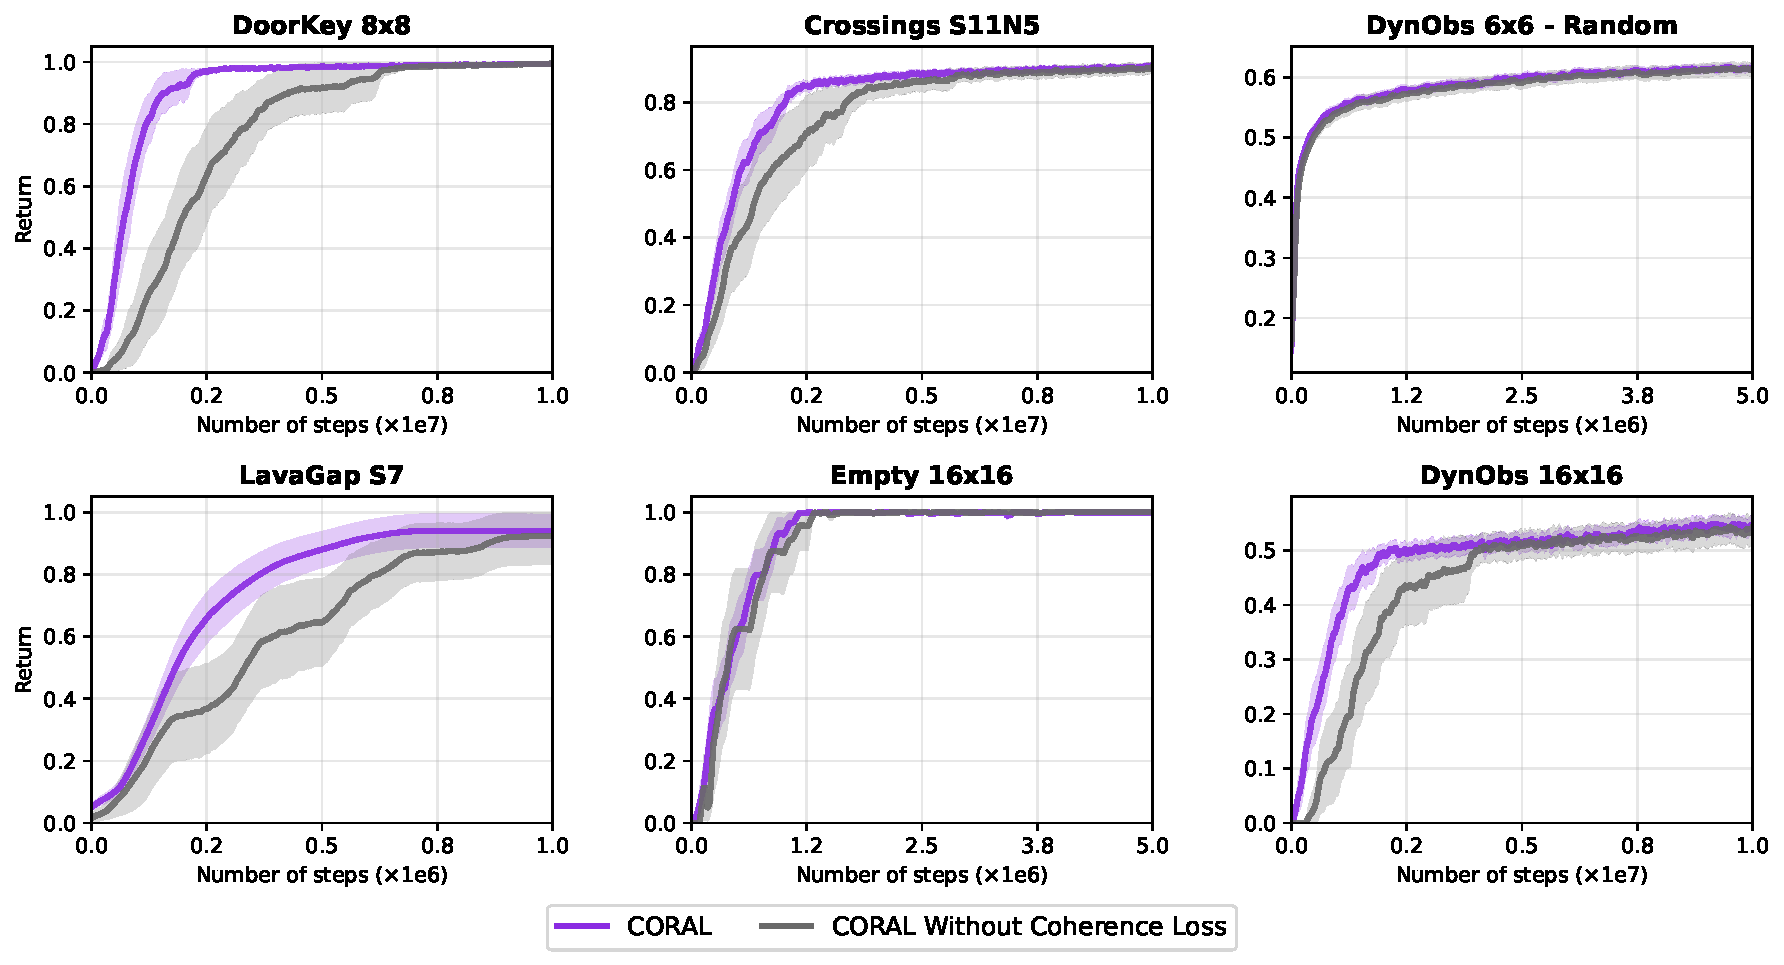
\includegraphics[width=.9\linewidth]{Figures/nocoh.pdf}
    \caption{\textbf{Ablation study on the Message Coherence Loss} Learning curves show the mean episodic return ($\pm95\%$ confidence interval) across 30 multiple seeds for a randomly initialized Control Agent paired with a pre-trained, frozen CORAL IA. \textcolor[HTML]{923BE5}{CORAL} demonstrates better sample efficiency and asymptotic performance compared to an ablated version where the Information Agent was pre-trained \textcolor[HTML]{696969}{without the Temporal Coherence Objective}. The consistent performance degradation in the ablated agent across unseen environments demonstrates that promoting temporal coherence in the communication protocol is critical for achieving better sample efficiency.}
    \label{fig:ablation_message_coh}
\end{figure*}
\newpage
\subsection{Information Agent Architecture}
Our Information Agent's design is based on a Transformer architecture to model the history of observations. We conducted an ablation study comparing it against a more traditional recurrent alternative. We implemented and pre-trained a version of the CORAL Information Agent where the Transformer block was replaced by a Gated Recurrent Unit (GRU) cell~\cite{chung2014empirical}. The GRU-based IA has comparable parameters and size, and is trained with the exact set of objectives as our main Transformer-based agent.
The in-context guided adaptation performance influenced by both architectures is presented in Table~\ref{fig:performance_GRU}. The resulting learning curves show that CORAL Transformer outperforms or matches CORAL GRU in all environments.
\begin{figure*}[!ht]
    \centering
    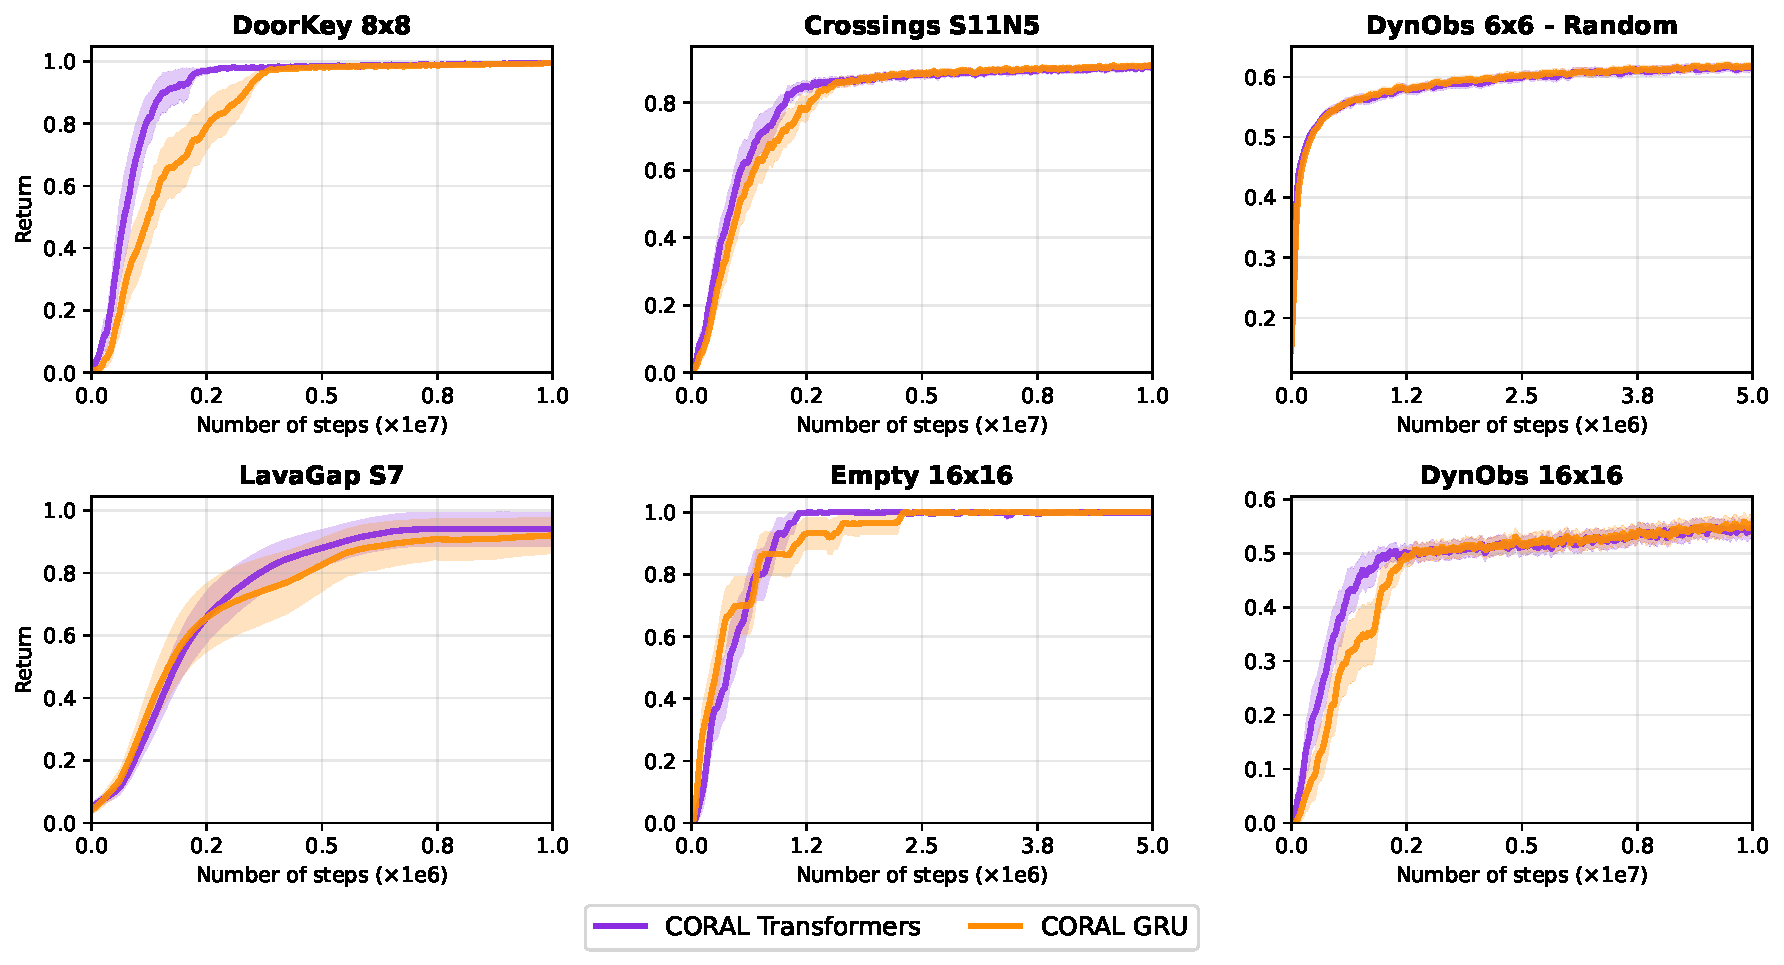
\includegraphics[width=.9\linewidth]{Figures/lc_gru_transformers.pdf}
    \caption{\textbf{Ablation study on the Information Agent's architecture.} Learning curves compare the in-context adaptation performance when the IA is implemented with a Transformer-based model versus a GRU-based alternative.}
    \label{fig:performance_GRU}
    \vspace{-5pt}
\end{figure*}
\newpage
\subsection{Message Dimensionality}
We performed an ablation study to analyze the sensitivity of CORAL to the dimensionality of the message vector. We pre-trained and deploy three versions of the framework using different message sizes: 16, 32, and 64, while keeping all other hyperparameters unchanged.
Table~\ref{fig:message_dim} shows that CORAL is relatively robust to this choice, with all variants learning efficiently, specially compared to the baselines studied in our experimental results. \textbf{Message Size of 32} consistently achieves the best or near-best performance across the majority of tasks. The performance of the agent using a message size of 16 is often marginally slower, while the largest size of 64 also exhibits a minor lag in learning speeds in several environments. Empirically, a message size of 32 demonstrated the most consistent performance, justifying its use in our main experiments.
\begin{figure*}[!ht]
    \centering
    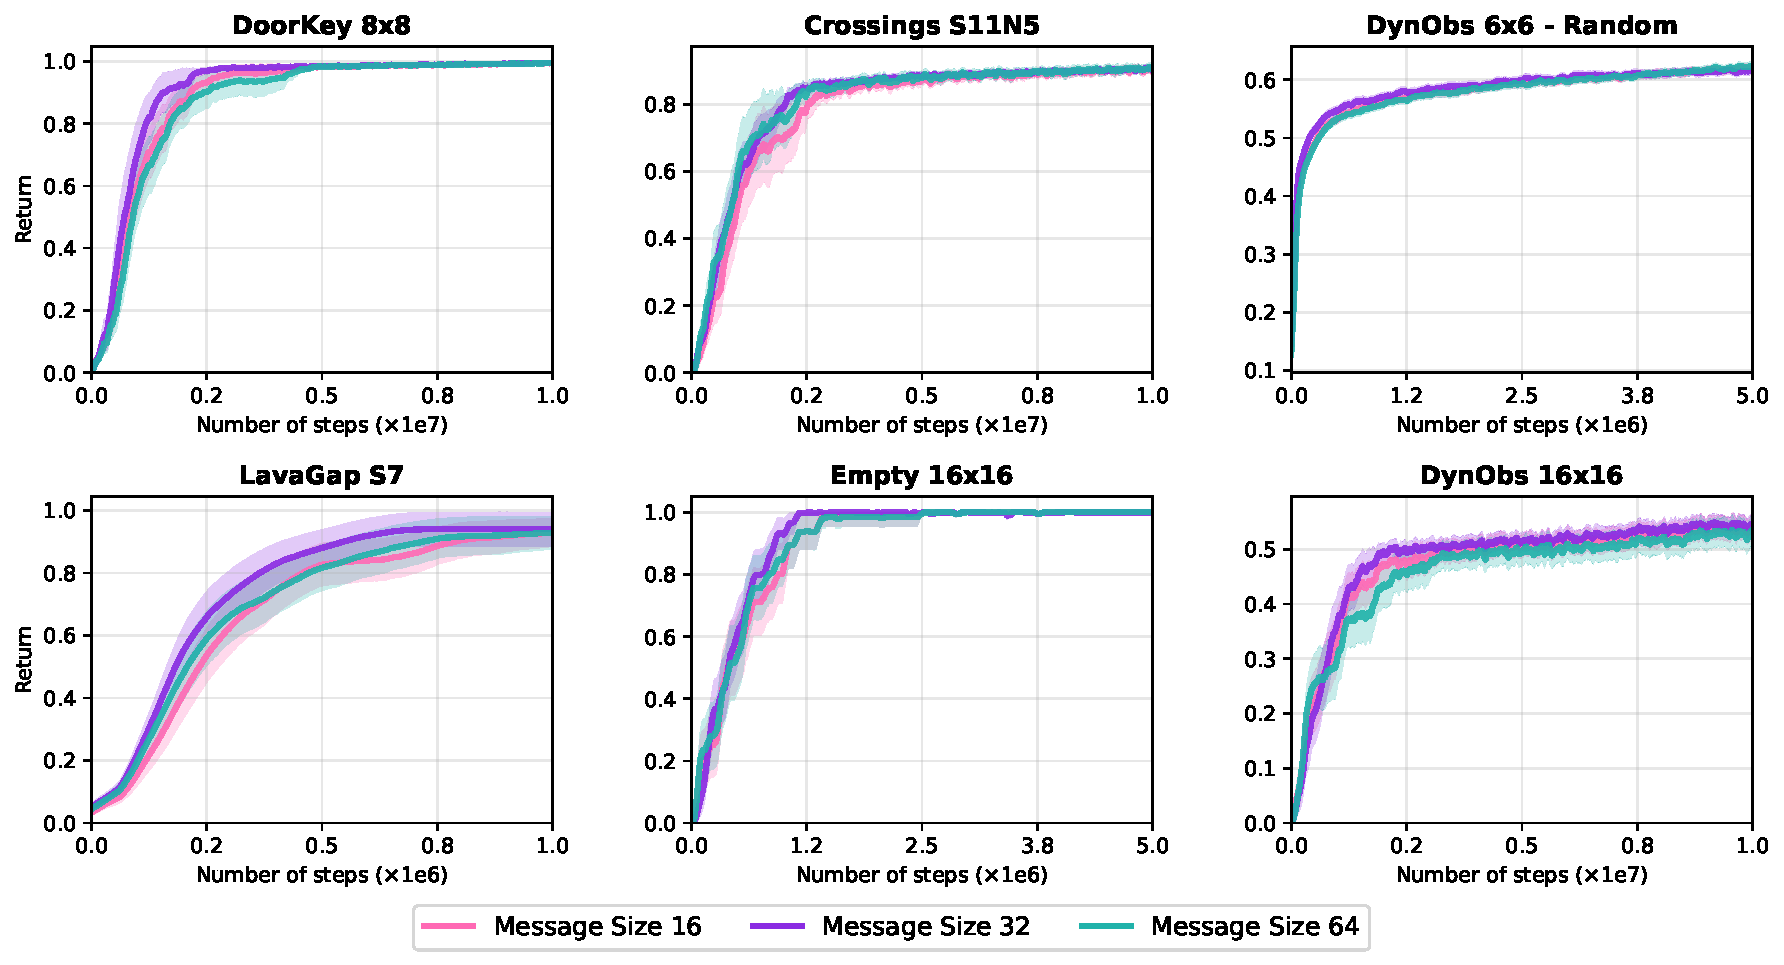
\includegraphics[width=.9\linewidth]{Figures/lc_vector_dim.pdf}
    \caption{\textbf{Ablation study on message dimensionality.} In-context adaptation performance of CORAL with different message vector sizes (16, 32, 64). While CORAL is robust to this hyperparameter, a message of size 32 consistently provides a slight performance advantage.}
    \label{fig:message_dim}
\end{figure*}
\end{appendix}
\end{document}
